%% ----------------------------------------------------------------------
%% START OF FILE
%% ----------------------------------------------------------------------

\chapter{相关技术简介}
\label{cha:related_work}

\section{存储介质简介}

\subsection{机械硬盘(HDD)}
机械硬盘(HDD,Hard Disk Driver)是最广泛使用的个人电脑非易失性存储设备,以覆盖有氧化铁的坚硬旋转盘片为存储介质。通过磁化盘面氧化铁单元的极性,机械硬盘在平整的磁性表面存储和检索数字数据。信息通过离磁性表面很近的读写磁头通过电流读写。每个盘片的存储面上都有一个磁头,所有的磁头联在一个磁头控制器上,由磁头控制器负责所有磁头的移动方向。磁头沿盘片的半径方向运动,加上盘片每分钟几千转的高速旋转,磁头就可以定位到盘片的指定位置进行盘片表面的数据读写操作。

机械硬盘的物理结构分为磁盘、磁头、电动机和主控芯片几部分。主电动机带动盘片旋转,副电动机带动磁头移动到碟片的某个位置,并决定读取磁盘正面或反面。磁头悬浮在磁盘上,磁盘旋转时就会画出一个与磁盘同心的圆形轨道(称磁道或柱面)。此时,磁头内部的磁感线圈感应磁盘上的磁铁极性,通过时间间隔定位扇区,读取/写入数据内容到当前磁头所处扇区。磁盘盘面以磁道、柱面和扇区的方式组织空间。

\begin{figure}[H]
\centering
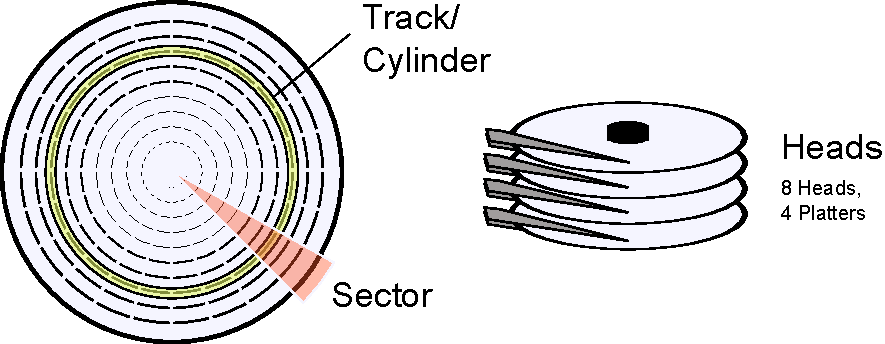
\includegraphics[width=0.6\linewidth]{./graph/hdd-struct}
\caption{机械硬盘结构}
\label{fig:hdd-struct}
\end{figure}

\begin{itemize}
\item 磁道
\\磁盘旋转时,磁头若保持在一个位置上,则每个磁头都会在磁盘表面划出一个圆形轨迹,这些圆形轨迹就叫做磁道(Track)。
\item 柱面
\\在有多个盘片构成的硬盘中,由不同盘片的面,但处于同一半径圆的多个磁道组成的一个圆柱面(Cylinder)。
\item 扇区
\\磁盘上的每个磁道被等分为若干个弧段,这些弧段便是硬盘的扇区(Sector)。硬盘的第一个扇区,叫做引导扇区。
\end{itemize}

机械硬盘盘片每分钟旋转圈数的单位是RPM(每分钟的转动数),存在4200、5400、5900、7200、10000、15000几种规格。转速越高数据传输速率愈快,但噪音、耗电量和发热量也会随之上升。

机械硬盘内部的盘片、磁头机械结构决定了机械硬盘擅长于顺序读写,随机读写性能较差。

\subsection{固态硬盘(SSD)}
固态硬盘(SSD,Solid State Driver)是一种基于永久性存储介质的存储器,如闪存,或非永久性存储介质的存储器,如同步动态随机存取存储器(SDRAM),的计算机外部存储设备。固态硬盘出现是为了代替传统机械硬盘。相比于机械硬盘,固态硬盘中已经没有了可以旋转的盘状结构,但是依照存储设备的命名习惯,这类存储器仍被称作硬盘。依据存储介质的类型,可分为易失性和非易失性两类。

\begin{enumerate}
\item 基于易失性记忆体的固态硬盘

由易失性记忆体作为存储介质的固态硬盘主要用于临时存储。易失性记忆体需要外界电力维持其内部的记忆功能,因此为了防止断电时的数据丢失,一般需要配合电池进行不间断供电。易失性存储介质,例如SDRAM,具有访问速度快(接近内存速度)、使用寿命长的特点。利用这一特点,可以将需要运行的程序首先从常规硬盘复制到固态硬盘中,然后交给计算机执行,由此可减少机械硬盘的启停延迟、寻道延迟对程序性能的影响。

此外,由易失性记忆体制成的固态硬盘还可用于应急备份。当电源意外中断时,靠电池驱动的固态硬盘可以有足够的时间将数据转移到非易失存储设备。电力恢复后,再从非易失存储设备中恢复数据。

\item 基于非易失性记忆体的固态硬盘

由非易失性记忆体作为存储介质的固态硬盘主在使用时和机械硬盘已经没有什么区别。非易失性存储介质(一般为NVRAM)的数据存取速度介于易失性介质和机械硬盘之间。和易失性介质相比,非易失性介质一经写入数据,无需外界电力来维持其记忆,不必考虑断电的影响使其更适于作为常规硬盘的替代品。

每块固态硬盘内部都会存在多个存储颗粒,每个存储颗粒中有非常多的存储单元储存数据。目前市面上主流的有三种NVRAM用作是固态硬盘的存储颗粒,分別是多层式储存颗粒(MLC,Multi Level Cell)、单层式储存颗粒(SLC,Single Level Cell)和三层式储存颗粒(TLC,Triple Level Cell)。SLC、MLC和TLC三者的区别是存储颗粒内部单个存储单元所能存储的状态个数:SLC一种,MLC两种,TLC三种。三者的读写速度差异不大。TLC主要用于制造企业级固态硬盘,使用MLC和TLC颗粒的固态硬盘的成本较使用SLC的低,但是寿命较短。

由于存储颗粒内部每个存储单元的写入次数是有限的,存储颗粒的最大写入次数便是存储颗粒的使用寿命。固态硬盘控制器通常会把写操作平均分配到存储颗粒内部的每个存储单元上,再通过映射表的方式定位数据的实际存储位置。工业界使用P/E cycle这一参数标准衡量固态硬盘的使用寿命,一个P/E cycle代表了固态硬盘内所有的存储颗粒被写入一次。固态硬盘的P/E cycle体现了硬盘内部存储颗粒可写入次数的峰值,P/E cycle越大固态硬盘的使用寿命越长。

\begin{table}[htb]
\centering
\caption{SLC、MLC和TLC的寿命和价格比较}
\begin{tabular}{|c|c|c|c|}
\hline  & SLC NAND Flash & MLC NAND Flash & TLC NAND Flash \\
\hline P/E Cycles & 100,000 & 10,000 & 4,000 \\
\hline Cell type & 1bit/cell & 2bit/cell & 3bit/cell \\
\hline Price (USD/GB) & 5 & 1.4 & 1 \\
\hline
\end{tabular}
\label{tab:slc-mlc-tlc-compare}
\end{table}

从表\ref{tab:slc-mlc-tlc-compare}可以看出,存储颗的粒密度从SLC到TLC逐渐增大,而P/E cycle逐渐减少。SLC颗粒常被用于生产企业级的固态硬盘,而MLC颗粒和TLC颗粒则较多的出现于桌面计算机的固态硬盘中。虽然TLC颗粒的P/E cycle与SLC颗粒存在将近两个数量级的差距,但实际应用情况表明,使用TLC存储颗粒的固态硬盘完全可以满足桌面计算机的使用寿命要求。

非易失性存储介质的固态硬盘并不是不存在缺点。在硬盘剩余空闲空间不多时,极有可能出现严重影响写入性能的Write cliff现象。Write cliff现象出现在当所有存储颗粒的空闲页都已经被初始化写入,新的写请求无法一次性得到足够的空闲页以完成写入操作的情况下。此时,固态硬盘控制器必须要擦除某些未写满的存储页面再进行写操作:控制器会将未写满存储页面的原有数据拷贝到临时空间,再进擦除;将原有数据与新数据进行合并,写入到擦除后的存储页面。拷贝原有数据到临时空间消耗的时间是Write cliff出现的主要原因。

固态硬盘厂商为了减少Write cliff对性能的影响,特别加入了针对固态硬盘的TRIM指令。当有文件需要被删除时,可通过TRIM指令会告知固态硬盘被删除文件的位置,固态硬盘控制器会将对应的存储块标记为空闲状态。这样,就能在一定程度上保证总是存在空闲页,从而降低Write cliff现象出现的概率。TRIM指令的出现,很大程度上提升了固态硬盘的性能、延长了固态硬盘的寿命,但当空闲页面无法满足写请求时,仍然需要擦除未写满的存储页面。因此,TRIM指令只能推迟而无法避免Write cliff现象的出现。
\end{enumerate}

\subsection{机械硬盘与固态硬盘的比较}
固态硬盘出现的目标是替代传统的机械硬盘,但是机械硬盘相较于固态硬盘的某些优势使得固态硬盘不可能在短期内动摇机械硬盘的统治地位。两者间的差距可以从以下几个方面进行比较。

\begin{enumerate}
\item 安全性
\\机械硬盘内部的盘片、电机等机械构造决定了在发生碰撞和震动时,磁头和盘片的接触往往会造成机械硬盘的损坏,从而导致数据的丢失。固态硬盘内部使用的缓存芯片几乎不受碰撞和震动的物理影响。
\item 性能
\\无论是启动速度还是读写速度,固态硬盘都有着非常明显的优势。造成这种优势的主要原因是固态硬盘没有磁头,不存在寻道时间。传统的机械硬盘则需要在指令接受后开始寻道。因此,固态硬盘在数据传输速度上要比普通机械硬盘有较大的优势。
\item 价格
\\2012年的统计数据表明,固态硬盘的价格是0.67美元/GB,传统的机械硬盘的价格是0.09美元/GB,固态硬盘价格是机械硬盘的7倍多。造成价格悬殊的主要因素是机械硬盘发展较早,技术相对成熟;固态硬盘技术则有待提高。固态硬盘的价格让很多用户望而却步,宁愿放弃速度而选择容量大的机械硬盘。
\item 容量
\\大数据时代的到来,带来了用户需日益增长的数据存储空间需求。大容量固态硬盘不仅非常稀少且价格昂贵,主流的固态硬盘一般都为128GB、256GB或512GB的存储空间。实际情况是,1TB的机械硬盘都已难以满足桌面电脑的需求,更不用说数据量巨大的企业级用户。
\item 耗电量
\\机械硬盘使用电机驱动盘片旋转和磁头移动,耗电量约为固态硬盘的3倍多。对于移动设备来讲,耗电量的多少关系到电池所能支持的待机时间的长短。在数据中心部署固态硬盘无疑可以节省大量的电能,从而节约电费支出。但基于DRAM的固态硬盘需要不间断供电,否则会导致数据丢失。
\item 重量和形状
\\由于不需要机械硬件的支持,固态硬盘的重量一般情况下仅有75-80克,而机械硬盘则高达700-750克,这使得移动设备可同时搭载多块固态硬盘。同时,固态硬盘内部结构的完全半导体化,使得其无结构样式限制,可根据实际需求设计成不同接口、形状的特殊固态硬盘。
\item 工作温度
\\由于固态硬盘采用闪存芯片存储数据,所以其在工作过程中产热相对较低。而机械硬盘由于高速的转速,盘片和空气的摩擦以及不同机械部件之间的摩擦产生比固态硬盘更多的热量,过高的温度容易影响到机械硬盘的工作状态。固态硬盘不但产热少而且能够适应10—70度的温度范围。
\item 噪音
\\ 固态硬盘得益于无机械部件及使用闪存芯片,不会产生任何噪音。而机械硬盘运行时则会产生一定的噪音,尤其是在企业硬盘组成的磁盘阵列中,更是需要专门的机房来存放磁盘阵列。
\end{enumerate}

\section{缓存技术}
\label{sec:cache_tech}

尽管自二十世纪九十年代以来,计算机硬件技术的发展带来了磁盘存储密度每半年到一年一倍的提升,但没有相应的技术能够以同样的速度缩短存储介质的访问时间。缓存技术作为一种减少IO子系统的响应时间、增加系统吞吐量的解决方案,已被广泛应用于存储子系统中。

\subsection{缓存的特点}
缓存中保存了主存储器中少部分数据的复制品,访问缓存的速度远高于主存储器。如果某个访问主存储器的请求,使用缓存中的数据就可以满足,就说缓存命中了一次。

由于缓存中保存的是主存储器中的部分数据,因此会出现找不到数据的情况,此时还是需要访问主存储器才能获得数据。如果这种情况发生的比例超过一定数值,缓存对系统性能的提升就无法得到保证。获得的主存储器数据被用来更新缓存数据内容,以便下次的数据访问不再需要到主存储器中获取。被频繁访问的数据并不是一成不变的,因此需要缓存页面替换算法不定期的更新缓存内的数据,这样才能保证缓存中的数据是被访问最频繁的,命中率才会有保证。

\subsection{缓存的工作原理}
为了形象说明缓存系统的工作原理,本小节会以CPU访问内存中的数据为例进行说明。绝大多数CPU中都集成了高速缓存以缩短访问内存的时间。

当CPU需要访问内存中的某个数据时,首先会从CPU缓存中查找,如果找到,就立即读取并传送给CPU进行处理;如果没有找到,就只能从速度相对较慢的内存中读取并传送给CPU进行处理,同时,把读取数据所在的数据块调入高速缓存中,这样做可以使以后对整块数据的读取都会在缓存中进行,避免了内存的访问。正是这种机制使CPU内部高速缓存的命中率非常高,大多数CPU可达到90\%左右,只有10\%的内存访问需要真正读取内存。这会大大节省访问内存的时间,也使CPU读取数据时基本无需等待。总的来说,CPU读取数据的顺序是先缓存后内存。

\subsection{缓存数据替换算法}
缓存系统运行过程中,需要对存储设备上的数据按照请求的频率进行冷热程度的划分,将经常访问的热数据存储在性能较高的存储设备上,将不经常访问的冷数据存储在性能较低的存储设备上,从而实现对不同热度数据的区别处理。缓存数据替换算法在缓存系统运行过程中,通过识别出的冷热数据,不断移动和更新缓存中数据,尽可能保证热数据存储在性能较高的存储设备,以达到提升缓存命中率和系统性能的目的。所以,从本质上讲,缓存数据替换算法就是冷热数据的识别算法。

从缓存数据替换算法的原理可以得出,冷热数据识别的准确率直接影响到了缓存系统的性能。学术上已经有很多关于热点数据的识别方法的研究成果。根据缓存空间组织的粒度,缓存数据替换算法可以分为两类,不同类型算法的识别的准确程度和计算复杂度会有不同。下面将逐一进行介绍。

\begin{enumerate}
\item 数据块级

数据块是最小的数据空间划分单位,通过数据块识别冷热数据需要将主存储空间和缓存空间按照相同大小的数据块进行划分。以数据块作为冷热程度的计数单位,根据数据块的访问频度,将频度高的数据块标记为热数据块。固态硬盘的内部设计中,数据块的热点识别主要用于固态硬盘的损耗平衡:通过一定的映射策略,将写操作平均分配到所有的存储块。

在数据块级进行冷热数据的识别的优势在于,它可以在微观层面精确地识别出真正的冷热数据块,同时又不必在考虑例如存储空间组织结构、文件系统等宏观的信息,从而简化了识别冷热数据的计算过程,保证了系统性能尽可能小的受计算复杂度的影响。

\item 文件级

文件级别的冷热数据划分是另一种缓存数据替换用到的判定方法。这种方法以文件作为热度统计的基本单位,为每个文件的设定保存热点程度的元数据,所有的文件访问操作都会对元数据中记录的热度值产生影响。文件级别的冷热数据划分可以从文件类型、文件大小、打开的文件句柄数目等多种宏观层面指标综合进行判别,提升判别的准确程度。

相比于数据块级别,文件级别可以有效减少元数据占用的空间,进而减少缓存系统额外的内存和数据消耗,而且还可以将数据块访问的随机性因素加入识别过程,更好的区分冷热数据文件。
\end{enumerate}


\subsection{缓存系统存在的目的}
缓存系统的存在通常是为了达到三个目标:
\begin{itemize}
\item 减少交互的通讯量:缓存数据能有效减少在进程和机器间的传输量。
\item 降低系统中的处理量:记录处理结果,减少重复处理的次数。
\item 降低主存储器的访问次数:如操作系统在内存中的缓存机械硬盘的数据。
\end{itemize}

在评估一个缓存系统的好坏时,一般会从性能、稳定性和可用性三个方面进行:
\begin{itemize}
\item 性能:定量分析缓存系统的命中率和缩短的延迟。
\item 稳定性:缓存算法本身是否稳定性,对于意外情况(如掉电),能否保证数据完整。
\item 可用性:系统对客户应是透明的,客户得到的仅仅是快速的响应和良好的可用性。
\end{itemize}

\section{混合存储系统}
\label{sec:hybrid_storage}

只要数据的处理速度和存储介质的访问速度、不同类型存储介质的访问速度仍然保持较大的差距,学术界和工业界就不会停止研究和探索利用不同速度的存储器件,搭建混合存储系统以提高系统的性能、容量和可靠性等指标。近二十年的研究已经获得了众多有价值的研究成果。

\subsection{基于DRAM与机械硬盘的混合存储}

使用DRAM作为机械硬盘的缓存一直是提高存储系统性能的重要手段之一。几乎所有操作系统在设计磁盘驱动程序时,都会优先考虑使用DRAM缓存机械硬盘的数据。硬盘制造商在制造硬盘时,同样会在硬盘控制器中加入8-16MB的DRAM芯片。利用数据的空间局部性原理,硬盘控制器在处理IO请求时读取的数据量会略大于请求的数据量,并在DRAM进行缓存。处于硬盘控制器中的DRAM缓存对于软件来说是透明的,磁盘驱动程序不必关心控制器缓存的运行情况。

但是采用DRAM作为缓存只能提高机械硬盘的读性能,对写性能的提高十分有限。这是因为,为了避免写入机械硬盘的脏数据由于掉电而丢失,磁盘控制器或是驱动程序就必须持续的将脏数据从易失性存储设备写入机械硬盘来保证数据的持久性。这使得缓存系统面临着数据可靠性和读写性能的两难选择,缓存越大性能提升越明显,脏数据在缓存中停留的时间也就会越长,数据因为掉电而丢失的可能性也就越大。基于以上原因的考虑,缓存系统都会限制缓存中脏数据的停留时间和数量。

\subsection{基于NVRAM与机械硬盘的混合存储}

基于NVRAM存储数据的非易失性,使得通过NVRAM缓存提升存储系统的写性能成为可能。常用的一种策略是将NVRAM与DRAM整合作为缓存,遇到写操作时,将数据同时写入NVRAM和DRAM,利用NVRAM的非易失性保证数据的可靠性,只有在系统掉电重启后NVRAM内的数据才会被访问,并重新写回到机械硬盘;另一种策略是将DRAM和NVRAM组合成单一的一个缓存空间,缓存块可以存储于任意的存储器中,所有的脏数据块必须存放在NVRAM上。

由于NVRAM的容量较小,因此带来的机械硬盘性能提升有限。虽然近年来NVRAM的容量的不断增大,但是相比于增长更为迅速的机械硬盘存储空间,加上大数据访问时呈现出的一次遍历的特征,使得基于NVRAM与机械硬盘的混合存储的NVRAM命中率不断下降,系统读写性能的提升效果不断减弱。

\subsection{高低转速磁盘的混合存储}

机械硬盘磁盘盘片的物理转速直接决定了读写请求处理的速度。利用不同规格、不同转速的机械硬盘来设计混合存储系统在20世纪90年代曾成为产业界研究的热点。

高低转速磁盘混合存储的基本思想是根据数据的访问频率、保留时间、重要性等指标,将频繁访问的热数据存储在转速为10000-15000 RPM的高速小容量SCSI机械硬盘中,而将访问频率低的冷数据存储在转速为5400-7200 RPM的低速大容量IDE/SATA 机械硬盘中。但由于机械硬盘本身机械原理的限制,不同转速机械硬盘之间的性能差距并不显著。因此,这种方法对存储系统的性能的提升非常有限。

\subsection{基于固态硬盘和机械硬盘的混合存储}

固态硬盘和机械硬盘之间性能的良好互补性,以及近几年高寿命、高密度的固态硬盘存储设备生产技术的日渐成熟,为设计高性能、低成本的混合存储系统提供了崭新的机遇。基于固态硬盘和机械硬盘的混合存储解决方案已成为大数据存储技术的新兴发展方向,并很快成为研究热点,其中企业存储解决方案提供商的发展尤其引人注目。Microsoft,LSI,Intel,EMC,IBM, Fusion-io等企业都已经或即将推出基于固态硬盘的混合存储解决方案。

\section{缓存算法评估}
\label{sec:cache_evaluation}

大多数学术论文在评估某种缓存算法的优劣时,都是只评估缓存的命中率。为了提高论文的说服力,有的还会给出该算法应用于某种环境所带来的性能提升比例。当工程师为混存系统挑选一种合适的缓存算法时,这些数据的参考价值都很有限,且不存在一种通用的评估方法。
下面介绍一种本论文提出并使用的缓存算法的评估模型,该模型既可以用于评估缓存算法给系统可能带来的性能提升,又可以为缓存系统工程师设计系统起到指导作用。

给出评估方法之前,式\ref{equ:cache_evaluation_syms}列出了推理中用到的数学符号。
\begin{equation}
\begin{split}
\\&T_1=\mbox{无缓存时,单个读/写请求处理时间}
\\&T_2=\mbox{有缓存且缓存命中时,单个读/写请求的处理时间}
\\&T_3=\mbox{有缓存但缓存时,单个读/写请求的处理时间}
\\&N=\mbox{读写请求总数量}
\\&R=\mbox{缓存命中率},R\in\lbrack0,1)
\\&T_q=\mbox{查询一个读/写请求在缓存池中是否命中的时长}
\\&T_c=\mbox{从缓存池拷贝或向缓存池写入完成一个读/写请求所需数据的时长}
\\&T_u=\mbox{使用单个未命中的读/写请求数据,更新缓存池所需时间}
\end{split}
\label{equ:cache_evaluation_syms}
\end{equation}

评估缓存对于系统IO性能的提升,可以用有、无缓存前提下,读写请求花费总时长的变化比例来表示。

\begin{equation}
\begin{split}
\mbox{性能提升比例}&=\frac{\mbox{无缓存条件下完成所有读写请求的总时长}}{\mbox{存在缓存时完成所有读写请求的总时长}}
\\&=\frac{NT_1}{NRT_2+N(1-R)T_3}
\\&=\frac{T_1}{RT_2+T_3-RT_3}
\\&=\frac{T_1}{T_3-(T_3-T_2)R}
\end{split}
\label{equ:cache_evaluation_enhance1}
\end{equation}

系统不存在缓存时,一个读/写请求所需的时间($T_1$)等同于该读/写请求直接应用于存储介质上所需的时间。

系统存在缓存且请求命中时,缓存系统利用缓存中数据即可完成读/写请求。这时,一个读/写请求所需的时间($T_2$)等同于查询缓存池所需时间($T_q$)加上从缓存池拷贝或向缓存池写入完成一个读/写请求所需数据的时间($T_c$)。
\begin{equation}
T_2=T_c+T_q
\end{equation}

系统存在缓存但未命中时,为了完成请求需要应用请求于存储介质,再使用获得的数据(读请求)或请求中包含的数据(写请求)更新缓存池。这时,一个读/写请求所需的时间($T_3$)等同于查询缓存池所需时间($T_q$),加上应用读/写请求于存储介质所需时间($T_1$),再加上使用新数据更新缓存池所需的时间($T_u$)。
\begin{equation}
T_3=T_q+T_1+T_u
\end{equation}

综上可以得出$T_2$与$T_3$的关系,同时,$T_3$也可以用$T_2$来表示(式\ref{equ:cache_evaluation_t2t3})。

\begin{equation}
T_3-T_2=T_1+T_u-T_c
\end{equation}
\begin{equation}
\label{equ:cache_evaluation_t2t3}
T_3=T_1+T_2+T_u-T_c
\end{equation}

最后,将式\ref{equ:cache_evaluation_t2t3}带入到提升比例计算公式\ref{equ:cache_evaluation_enhance1},得出最终的性能提升比例计算公式\ref{equ:cache_evaluation_enhance2}。

\begin{equation}
\begin{split}
\mbox{性能提升比例}&=\frac{T_1}{T_3-(T_3-T_2)R}
\\&=\frac{T_1}{(T_1+T_2+T_u-T_c)-(T_1+T_u-T_c)R}
\\&=\frac{T_1}{T_2+(T_1+T_u-T_c)(1-R)}
\\&=\frac{T_1}{T_q\textdownarrow+T_c+(T_1+T_u\textdownarrow-T_c)(1-R\textuparrow)}\textuparrow
\end{split}
\label{equ:cache_evaluation_enhance2}
\end{equation}

$T_1$取决于被缓存储介质的性能;$T_c$取决于缓存存储介质的性能。这两个值在硬件环境一定的情况下为定值。

提升缓存系统性能就是提高缓存系统为原系统带来的性能提升比例。式\ref{equ:cache_evaluation_enhance2}表明,可以从以下三个点着手:

\begin{enumerate}
\item
提高缓存池的查询速度,缩短查询时间$T_q$。
\item
提高缓存池的更新速度,缩短更新时间$T_u$。
\item
优化缓存算法,提高缓存命中率$R$。
\end{enumerate}

从工程的经验角度讲上面的三个着手点也是行得通的。

%% ----------------------------------------------------------------------
%%% END OF FILE
%% ----------------------------------------------------------------------